% https://tex.stackexchange.com/a/357657
\documentclass{beamer}
\usepackage{animate}
\usepackage{tikz}
\usepackage[utf8]{inputenc}
\usetikzlibrary{matrix}

\begin{document}
\begin{frame}[fragile]
  \begin{animateinline}[step,controls]{1}
    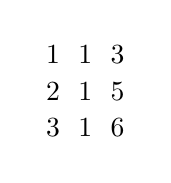
\begin{tikzpicture}
      \matrix (magic) [matrix of nodes]
      {
        1 & 1 & 3  \\
        2 & 1 & 5  \\
        3 & 1 & 6  \\
      };
    \end{tikzpicture}
  \newframe
    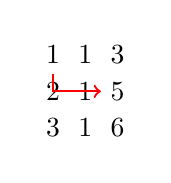
\begin{tikzpicture}
      \matrix (magic) [matrix of nodes]
      {
        1 & 1 & 3  \\
        2 & 1 & 5  \\
        3 & 1 & 6  \\
      };
      \draw[thick,red,->] (magic-1-1) |- (magic-2-3);
    \end{tikzpicture}
  \end{animateinline}
\end{frame}
\end{document}
